
\section{Ciclo biológico del Aedes Aegypti}
\label{sec:caracteristicas-biologicas}
De todas las especies de mosquitos conocidos, con importancia en salud pública, Aedes Aegypti,
es considerada la más peligrosa por tener la capacidad de transmitir el mayor número de
enfermedades arbovirales\footnote{Las infecciones arbovirales son los virus que se transmiten por
los mosquitos. \textit{Arbo} es una abreviatura que significa transmitida por los artrópodos, los
cuales son insectos.}, al hombre \cite{ThironIzcazaJ2003}.

Los sitios de cría del Aedes aegypti son fundamentalmente artificiales: urbanos (en baldíos,
cementerios, desarmaderos, basurales) o domésticos (neumáticos, floreros, botellas, bebederos de
animales, latas abiertas o contenedores de cualquier tipo, depósito de agua de bebida, cisternas,
vasijas, tinajas, todo tipo de recipientes en desuso, aun pequeños, prácticamente de cualquier
objeto que retenga agua) \cite{directricesDetvArg}.

Prefieren agua limpia, con bajo tenor orgánico y de sales disueltas. La puesta de huevos la
realizan en la superficie del recipiente. Algunos recipientes le son más atractivos que otros, en
especial los de color oscuro, de boca ancha, que están al nivel del suelo y se encuentran en la
sombra \cite{ThironIzcazaJ2003}.


Su ciclo de vida manifiesta una metamorfosis completa, es decir que las formas inmaduras salidas
del huevo son completamente diferentes al adulto, las primeras son de vida acuática, las segundas
de vida aérea \cite{directricesDetvArg}, donde su desarrollo se encuentra dividido en cuatro
etapas, huevo, larva, pupa y adulto \cite{web-site:gMonteroBiologia}
(\figref{fig:cap3-ciclo-de-vida}).

\begin{figure}[H]
\centering
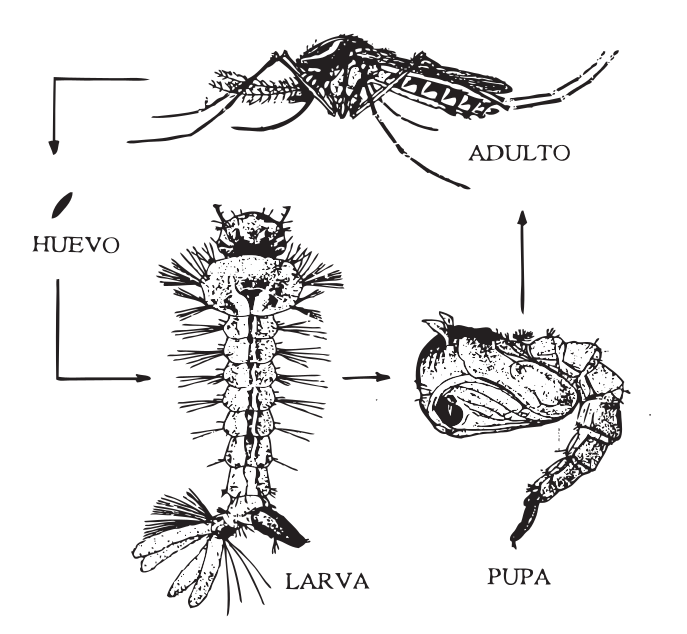
\includegraphics[width=0.7\textwidth]{capitulo-3/graphics/ciclo-de-vida.png}
\caption{\label{fig:cap3-ciclo-de-vida} Ciclo de vida del Aedes Aegypti (Tomado de
\cite{directricesDetvArg}).}
\end{figure}

\subsection{Huevo}
\label{subsec:ciclo-biologico-huevo}
Los huevos miden aproximadamente un milímetro de longitud, son depositados uno a uno al ras del
agua quedando adheridos a las paredes del recipiente \cite{ThironIzcazaJ2003}. Cada vez que sube el
nivel del agua en el recipiente eclosiona un grupo de huevos, de este modo, se aseguran una
eclosión escalonada que permite la supervivencia aún en condiciones desfavorables
\cite{directricesDetvArg}.

\begin{figure}[H]
\centering
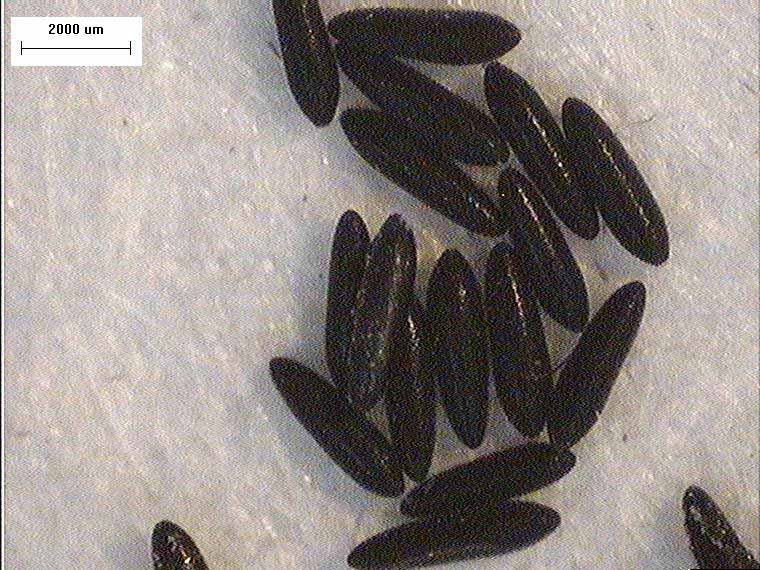
\includegraphics[width=0.5\textwidth]{capitulo-3/graphics/huevos.png}
\caption{\label{fig:cap3-huevos} Huevos del mosquito Aedes Aegypti (Tomado de
\cite{sivanathan2006ecology}).}
\end{figure}

Al momento de la postura son de coloración blanca, casi transparentes, en contacto con el aire van
adoptando la coloración oscura característica \cite{directricesDetvArg} (\figref{fig:cap3-huevos}).
La fecundación ocurre al momento de la postura del huevo, en donde el desarrollo embrionario
transcurre en alrededor de 48 horas si el ambiente es húmedo y cálido, si la temperatura es baja
se prolonga hasta por cinco días \cite{ThironIzcazaJ2003}. Los huevos son formas de resistencia que
pueden sobrevivir durante muchos meses en clima adverso hasta que las condiciones ambientales
favorezcan su eclosión \cite{directricesDetvArg}.

\subsection{Larva}
\label{subsec:ciclo-biologico-larva}
Los huevos eclosionan dando lugar a formas larvarias, acuáticas, nadadoras, de respiración aérea
\cite{directricesDetvArg} y es el período de mayor alimentación y crecimiento
\cite{web-site:gMonteroBiologia}. Pasan la mayor parte del tiempo alimentándose del material
orgánico sumergido o acumulado en las paredes y el fondo del recipiente
\cite{web-site:gMonteroBiologia, directricesDetvArg}.

Las larvas que emergentes inician un ciclo de 4 estadios larvales \cite{web-site:gMonteroBiologia},
donde, estos estadios definen su período de crecimiento y desarrollo \cite{ThironIzcazaJ2003}. El
primer estadio larval es la forma que emerge del huevo, transcurre en uno o dos días que ha
dedicado a alimentarse y a crecer; ocurre la muda y surge el segundo estadio
\cite{ThironIzcazaJ2003}. En el segundo estadío, la cápsula cefálica y el sifón son blandos y
transparentes, al extenderse permite el subsecuente desarrollo, se endurecen y oscurecen
\cite{ThironIzcazaJ2003}. Después del segundo estadio, la cápsula cefálica y el sifón no cambian
de tamaño, el tórax y el abdomen crecen considerablemente durante cada fase
\cite{ThironIzcazaJ2003}.

\begin{figure}[H]
\centering
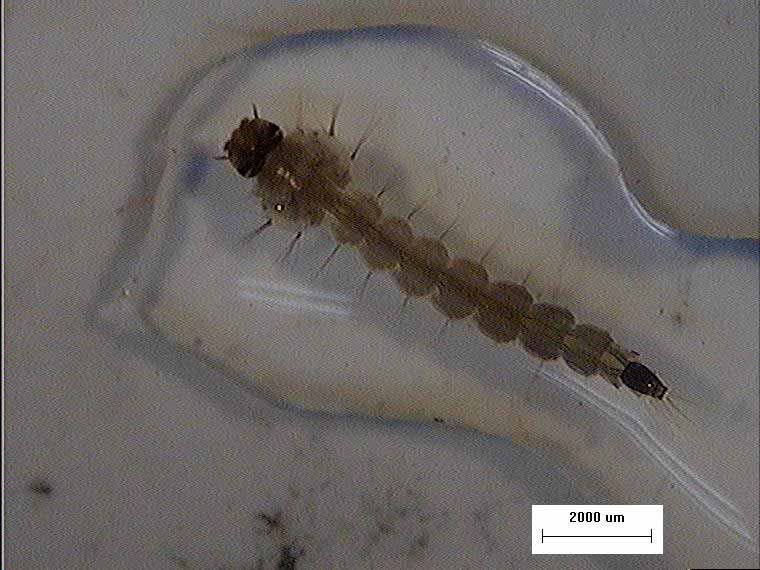
\includegraphics[width=0.5\textwidth]{capitulo-3/graphics/larva.png}
\caption{\label{fig:cap3-larvas} Larva del mosquito Aedes Aegypti (Tomado de
\cite{sivanathan2006ecology}).}
\end{figure}

La duración del desarrollo larval está en función de la temperatura, la disponibilidad de alimento
y la densidad de larvas en el criadero \cite{ThironIzcazaJ2003}. Los primeros tres estadios se
desarrollan rápidamente, mientras que el cuarto toma más tiempo, debido a que aumenta
considerablemente su tamaño y peso \cite{ThironIzcazaJ2003, web-site:gMonteroBiologia},
en condiciones de baja temperatura o escasez de alimento el cuarto estadio puede prolongarse por
varias semanas \cite{ThironIzcazaJ2003}. En condiciones óptimas, el período larval desde la
eclosión hasta la pupación puede ser de cinco días, pero por lo regular ocurre de siete a catorce
días \cite{ThironIzcazaJ2003}.

La mortalidad, más elevada ocurre frecuentemente en los primeros estadios larvales
\cite{ThironIzcazaJ2003}, donde la principal causa es atribuida a la inestablididad de los
criaderos que sirven como habitad.

\subsection{Pupa}
\label{subsec:ciclo-biologico-pupa}
Las pupas, al igual que las larvas, son acuáticas, estas no se alimentan, su función es la
metamorfosis del estadio larval al adulto \cite{ThironIzcazaJ2003}. El período pupal dura de 1
a 3 días en condiciones favorables, con temperaturas entre 28 y 32 \textcelsius
\cite{web-site:gMonteroBiologia}, emergiendo alrededor del 88\% de los adultos en cuestión de 48
horas \cite{ThironIzcazaJ2003}. Las variaciones extremas de temperatura pueden dilatar este período
\cite{web-site:gMonteroBiologia}.

\begin{figure}[H]
\centering
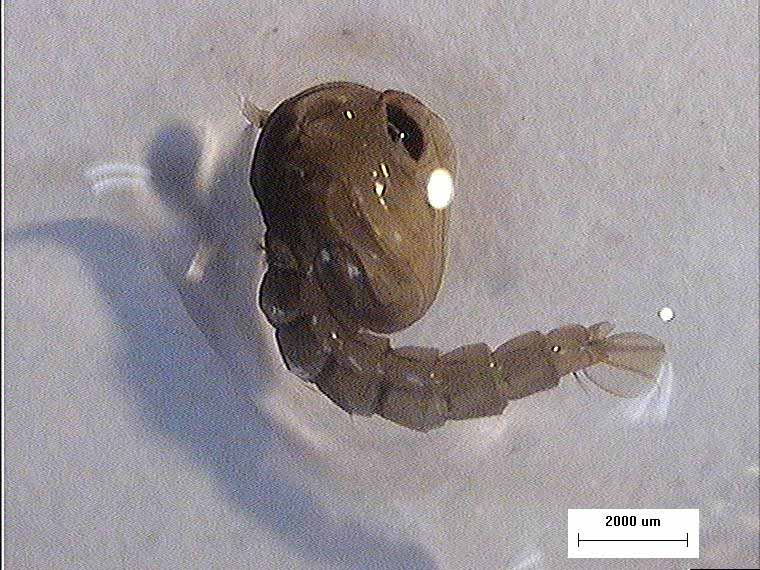
\includegraphics[width=0.5\textwidth]{capitulo-3/graphics/pupa.png}
\caption{\label{fig:cap3-larvas} Larva del mosquito Aedes Aegypti (Tomado de
\cite{sivanathan2006ecology}).}
\end{figure}

\subsection{Adulto}
\label{subsec:ciclo-biologico-adulto}
La función más importante del adulto es la reproducción \cite{ThironIzcazaJ2003}. Aproximadamente
la mitad de los adultos emergentes son hembras \cite{otero2006stochastic, manrique1998desarrollo}.
Los adultos recién emergidos permanecen las primeras 24 horas en fase teneral, tiempo en que se
efectúa el endurecimiento y obscurecimiento de su cutícula \cite{luevano1993ciclo}. Pueden
permanecer vivos en el laboratorio durante meses y en la naturaleza pocas semanas, con una
mortalidad diaria de 10\%, la mitad de los mosquitos morirán durante la primera semana y 95\% en
el primer mes \cite{ThironIzcazaJ2003}.

\begin{figure}[H]
\centering
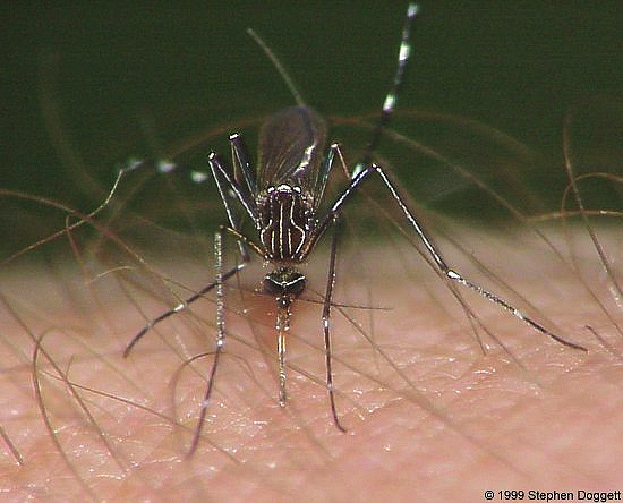
\includegraphics[width=0.5\textwidth]{capitulo-3/graphics/adulto.png}
\caption{\label{fig:cap3-larvas} Adulto del mosquito Aedes Aegypti (Tomado de
\cite{directricesDetvArg}).}
\end{figure}

Las partes bucales del macho no están adaptadas para chupar sangre, se alimentan de carbohidratos
de cualquier fuente accesible como frutos o néctar de flores que satisface sus requerimientos
energéticos \cite{ThironIzcazaJ2003}. Las hembras también se alimentan de esta misma fuente como
complemento indispensable, sin embargo necesitan alimentarse de sangre para obtener las proteínas
necesarias para la formación de los huevos \cite{ThironIzcazaJ2003}.

Antes de 24 horas ambos sexos están listos para el apareamiento, alrededor del 58\% de las hembras
nulíparas \footnote{Nulíparas son aquellas hembras jóvenes que no han ovipuesto.} son inseminadas
antes de su primera alimentación sanguínea, un 17\% durante y el 25\% es inseminada entre la
segunda alimentación y la primera oviposición \cite{ThironIzcazaJ2003}. Una inseminación es
suficiente para fecundar todos los huevos que la hembra produzca en toda su vida
\cite{ThironIzcazaJ2003}. El apareamiento que por lo general se efectúa durante el vuelo debido a
que el macho es atraído por  el sonido emitido por las alas de la hembra \cite{ThironIzcazaJ2003}.
El patrón diario de alimentación de los mosquitos, varia de acuerdo a las localidades y subespecies
\cite{luevano1993ciclo}.

Los mosquitos tienen la particularidad de volar en sentido contrario al la dirección al viento a
una velocidad máxima de $2 km/h$ \cite{web-site:speedAnimals}.  Por sus hábitos, es considerado
como doméstico \cite{luevano1993ciclo}, tiende a permanecer en el lugar en donde emergió
\cite{cabezas2005dengue,ThironIzcazaJ2003}, siempre y cuando no exista algún factor que la
perturbe o no disponga de huéspedes, sitios de reposo y de postura  \cite{ThironIzcazaJ2003}. Por
lo general mosquito no sobrepasa los 50 a 100 metros durante su vida \cite{cabezas2005dengue}. Los
sitios de cría del Aedes aegypti son fundamentalmente artificiales o domésticos
\cite{directricesDetvArg}. En caso de no haber recipientes adecuados, la hembra grávida es capaz
de volar hasta tres kilómetros en busca de este sitio \cite{ThironIzcazaJ2003}.

Es común que después de cada alimentación sanguínea la hembra desarrolle un lote de huevos, la
cantidad de huevos depende de la alimentación que puede variar entre 100 a 200 huevos
\cite{cabezas2005dengue}. El intervalo de tiempo que transcurre entre la alimentación sanguínea y
la postura, denominado ciclo gonotrófico, es de 48 horas en los trópicos bajo condiciones óptimas
de temperatura\cite{ThironIzcazaJ2003}. Dentro de la bionomía de vectores, una fase muy importante
es el ciclo gonotrófico, el cual es un proceso fisiológico que consiste en la digestión de la
comida sanguínea y desarrollo de los ovarios \cite{luevano1993ciclo}.
